\documentclass[a4paper,10pt]{article}
\usepackage[margin=30mm]{geometry}

% language
\usepackage[utf8]{inputenc}
\usepackage[english]{babel}
\usepackage{amsmath}
\usepackage{parskip}
\usepackage{mathtools}
% colors
\usepackage{xcolor}
\definecolor{code_bg}{rgb}{0.95,0.95,0.92}

% code sections
\usepackage{listings}
\lstset{
  language=C,
  backgroundcolor=\color{code_bg},
  numbers=left,
  numbersep=5pt,
  numberstyle=\tiny\color{gray},
  captionpos=b,
  framexleftmargin=12pt,
  framextopmargin=2pt,
  framexbottommargin=2pt, 
  frame=tb, framerule=0pt,
  aboveskip=0pt,
  belowskip=1em,
  xleftmargin=4.5mm,
}

\usepackage{graphicx}         % includegraphics{}
\usepackage{float}            % H placement for figures
\usepackage{amsmath}          % matrix

\renewcommand\thesection{\Alph{section}}
\renewcommand\thesubsection{\Alph{section}\arabic{subsection}}

\newcommand{\task}[1]{{\bf #1}}

\begin{document}
\begin{center}
  \textbf{\Huge TU Berlin Robotics WiSe 18/19} \\
  \textbf{\huge Lab Assignment \#2}
\end{center}

\vfill

\begin{figure}[H]
  \centering
  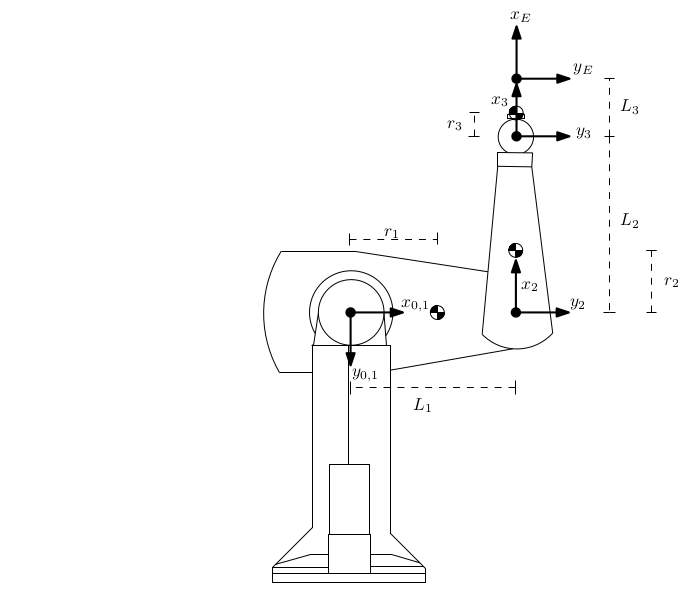
\includegraphics[scale=1.9]{img/robot_arm.png}
  \caption{RRR Puma in zero configuration}
\end{figure}

\begin{table}[h!]
  \begin{center}
    \begin{tabular}{c|c|c|c|c|c|c}
      Joint: & 1 & 2 & 3 & 4 & 5 & 6\\\hline
      $\tau_{max}$: & 97,6 Nm & 156,4 Nm & 89,4 Nm & 24,2 Nm & 20,1 Nm & 21,2 Nm
    \end{tabular}
    \caption{torque limits of the PUMA robot}
  \end{center}
\end{table}

\vfill

\begin{table}[h!]
  \begin{center}
    \begin{tabular}{rccccccccccc}
               ~          & \textbf{A1} & \textbf{A2} & \textbf{A3} & \textbf{(A4)} & \textbf{(B1)} & \textbf{B2} & \textbf{C1} & \textbf{C2} & \textbf{C3} & \textbf{C4} & \textbf{C5}\\\hline
      Jiaqiao Peng        &      ~      &      ~      &      ~      &       ~       &       ~       &      ~      &      ~      &      ~      &      ~      &      ~      &      ~     \\\hline
      Benjamin Oesterle   &      ~      &      ~      &      ~      &       ~       &       ~       &      ~      &      ~      &      ~      &      ~      &      ~      &      ~     \\\hline
      Botond Péter Sléber &      ~      &      ~      &      ~      &       ~       &       ~       &      ~      &      ~      &      ~      &      ~      &      ~      &      ~     \\\hline
      Dhananjay Mukhedkar &      ~      &      ~      &      ~      &       ~       &       ~       &      ~      &      ~      &      ~      &      ~      &      ~      &      ~     \\\hline
      
    \end{tabular}
    \caption{implementation table (we solved all tasks as a group)}
  \end{center}
\end{table}

\newpage

\section{Forward Kinematics}

\subsection{Transformation Between Frames}
$\prescript{0}{E}{T}=\prescript{0}{1}{T} \prescript{1}{2}{T} \prescript{2}{3}{T} \prescript{3}{E}{T}=
$$
\begin{pmatrix} 
c_1 & -s_1  & 0 & 0\\
s_1 & c_1 & 0 & 0 \\
0 & 0 & 1 & 0 \\
0 & 0 & 0 & 1 
\end{pmatrix}
\cdot
\begin{pmatrix} 
s_2 & c_2 & 0 & L_1 \\
-c_2 & s_2 & 0 & 0 \\
0 & 0 & 1 & 0 \\
0 & 0 & 0 & 1
\end{pmatrix}
\cdot
\begin{pmatrix} 
c_3 & -s_3 & 0 & L_2 \\
s_3 & c_3 & 0 & 0 \\
0 & 0 & 1 & 0 \\
0 & 0 & 0 & 1
\end{pmatrix}
\cdot
\begin{pmatrix} 
1 & 0 & 0 & L_3 \\
0 & 1 & 0 & 0 \\
0 & 0 & 1 & 0 \\
0 & 0 & 0 & 1
\end{pmatrix}
$$
$

$
\prescript{0}{E}{T}=
\begin{pmatrix} 
c_3 & -s_3 & 0 & c_3L_3+L_2 \\
s_3 & c_3 & 0 & s_3L_3 \\
0 & 0 & 1 & 0 \\
0 & 0 & 0 & 1
\end{pmatrix}
$
\\~\\

\subsection{End Effector Position In Operational Space}

The end-effector position and orientation is calculated:

$
\prescript{0}{E}{T}(q)\cdot
\begin{pmatrix} 
0 \\
0 \\
0 \\
1
\end{pmatrix}_{EE}
=
\begin{pmatrix} 
c_1L_1 + s_{12}L_2 + s_{123}L_3 \\
s_1L_1 - c_{12}L_2 - c_{123}L_3 \\
0 \\
1
\end{pmatrix}
$

End effector orientation:
$
\theta = q_1+q_2+q_3- \frac{\pi}{2}
$
\\~~\\
Finally, 

$
F(q)=
\begin{pmatrix}
c_1L_1+s_{12}L_2+s_{123}L_3 \\
s_1L_1 - c_{12}L_2 - c_{123}L_3\\
q_1+q_2+q_3- \frac{\pi}{2}
\end{pmatrix}
$
\\~\\
\subsection{Compute The End Effector Jacobian}

End effector Jacobian:

$$
\dfrac{\partial J(q)}{\partial q} = 
\begin{pmatrix}
-s_1L_1+c_{12}L_2+c_{123}L_3 & c_{12}L_2+c_{123}L_3 & c_{123}L_3 \\
c_1L_1 + s_{12}L_2 + s_{123}L_3 & s_{12}L_2 + s_{123}L_3 & s_{123}L_3\\
1 & 1 & 1
\end{pmatrix} 
$$

\subsection{Understanding The Jacobian Matrix And Pose Singularities}

\subsection*{a)}
\begin{figure}[H]
	\begin{center}
		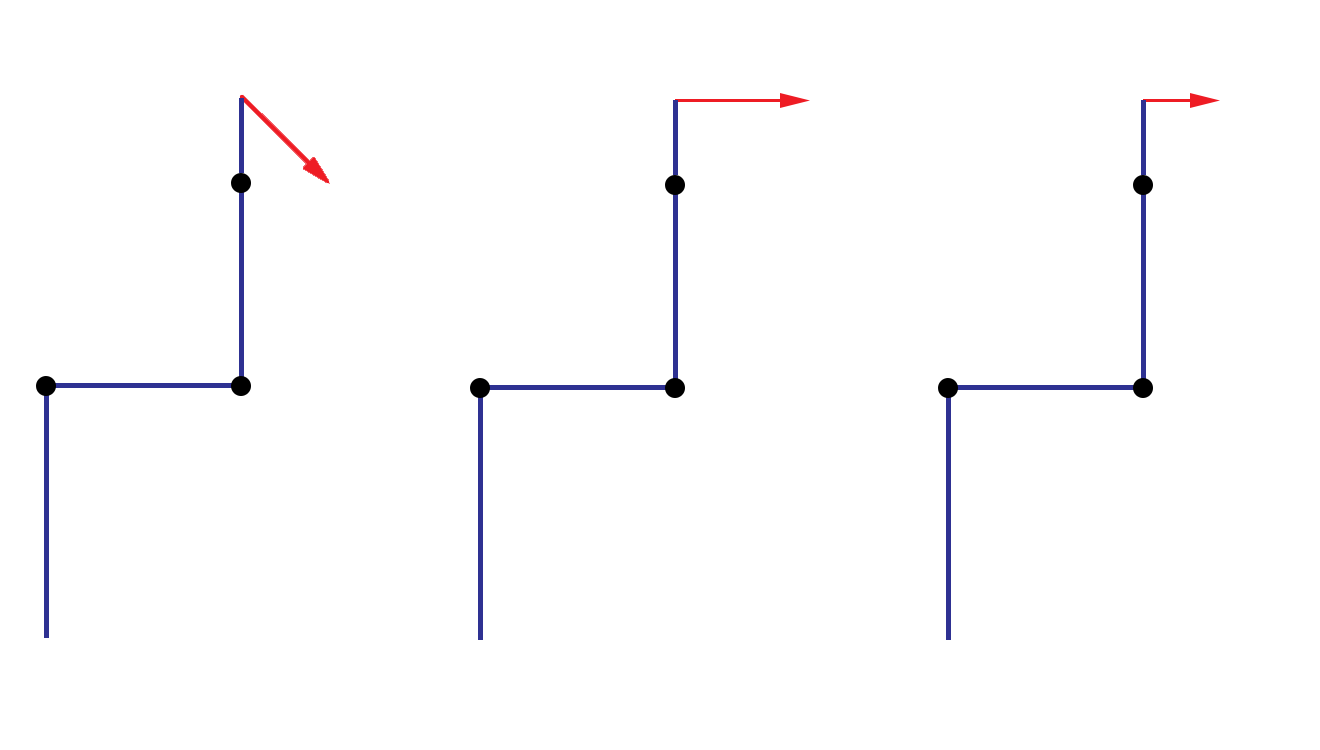
\includegraphics[scale=0.3]{img/1_full.png}
	\end{center}
\end{figure}
EE velocity, when 
$
\dot{q}_{11} =
\begin{pmatrix}
1 & 0 & 0
\end{pmatrix}
\dot{q}_{12} =
\begin{pmatrix}
0 & 1 & 0
\end{pmatrix}
\dot{q}_{13} =
\begin{pmatrix}
0 & 0 & 1
\end{pmatrix}
$
and  
$
q_1=
\begin{pmatrix}
	0 & 0 & 0
\end{pmatrix} 
$
\\~\\
\begin{figure}[H]
	\begin{center}
		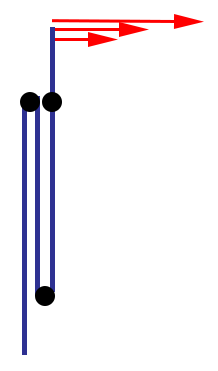
\includegraphics[scale=0.3]{img/2_full.png}
	\end{center}
\end{figure}
EE velocity, when 
$
\dot{q}_{21} =
\begin{pmatrix}
1 & 0 & 0
\end{pmatrix}
\dot{q}_{22} =
\begin{pmatrix}
0 & 1 & 0
\end{pmatrix}
\dot{q}_{23} =
\begin{pmatrix}
0 & 0 & 1
\end{pmatrix}
$
and  
$
q_2=
\begin{pmatrix}
\frac{\pi}{2} & -\frac{\pi}{2} & 0
\end{pmatrix}
$

$
| \dot{q}_{21} |>|\dot{q}_{22}|>|\dot{q}_{23}| 
$
\\~\\
\begin{figure}[H]
	\begin{center}
		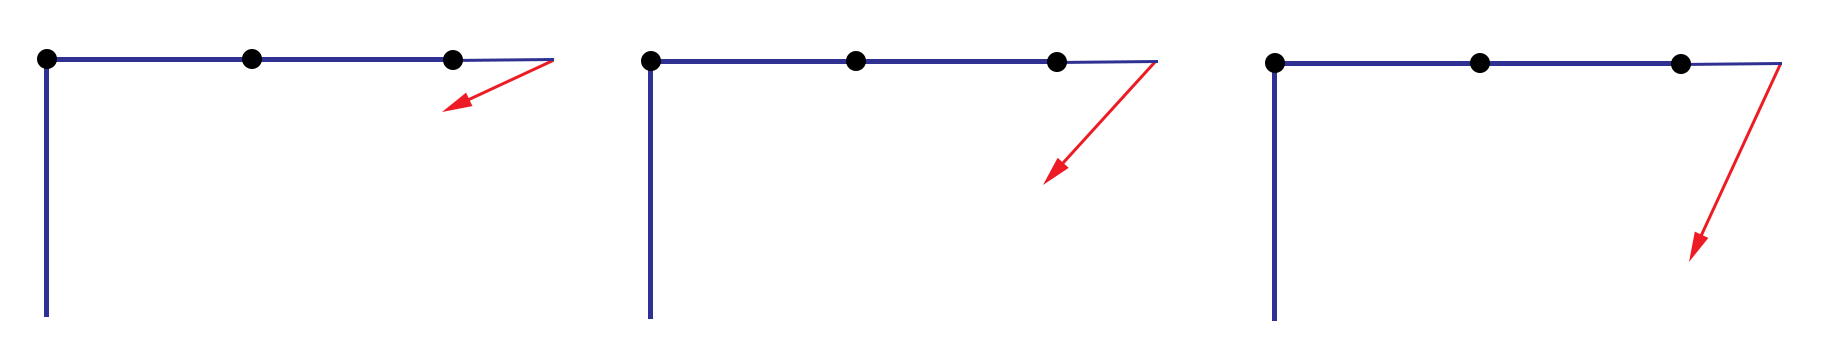
\includegraphics[scale=0.3]{img/3_full.png}
	\end{center}
\end{figure}
EE velocity, when 
$
\dot{q}_{31} =
\begin{pmatrix}
0 & 0 & 1
\end{pmatrix}
\dot{q}_{32} =
\begin{pmatrix}
0 & 1 & 0
\end{pmatrix}
\dot{q}_{33} =
\begin{pmatrix}
1 & 0 & 0
\end{pmatrix}
$
and  
$
q_3=
\begin{pmatrix}
0 & \frac{\pi}{2} & 0.01
\end{pmatrix} 
$
\\~\\
\subsection*{b)}

In the first case the robot is not in a singularity. The robot has all degrees of freedom.\\

In the second case, all the velocities are paralell, so the robot is in a singularity. The robot cannot move in y direction.\\

In the third case, nearly all velocities are in the same direction, so the robot is close to singularity.
\newpage



\section{Trajectory Generation In Joint Space}

\subsection{Generation Of Smooth Trajectories With Polynomial Splines}
\subsection*{a)}
Zero configuration:
$q_a =
\begin{pmatrix}
	0,&0,&0
\end{pmatrix}^T
$

Intermediate point:
$q_b = 
\begin{pmatrix}
-\frac{\pi}{4}, &\frac{\pi}{2}, &0
\end{pmatrix}^T
$

Final configuration:
$q_c =
\begin{pmatrix}
-\frac{\pi}{2},&\frac{\pi}{4},&0
\end{pmatrix}^T
$
\\~\\
Two splines:

$
u_1(t) = a_0 +a_1t_{via} + a_2 t_{via}^2 + a_3 t_{via}^3\\
u_2(t) = b_0 +b_1(t-t_{via}) + b_2 (t-t_{via})^2 + b_3 (t-t_{via})^3
$
\\~\\
Contraints:

$q(0)=q_0$

$q(t_f)=q_f$

$\dot{q}(0)=0$

$\dot{q}(t_f)=0$



Velocities at the intermediate point:

$\dot{q}_b(t_f)=
\begin{pmatrix}
-\frac{\pi}{10},&0,&0
\end{pmatrix}^T [\frac{rad}{s^2}]
$
\\~\\
Equations for computing the for the scalar values:
\\~\\
$a_0=q_0$

$a_1=\dot{q_0}$

$a_2=\frac{3}{t_{via}^2}(u_{via}-u_0)-\frac{2}{t_{via}}\dot{u}_0-\frac{1}{t_{via}}\dot{u}_{via}$

$a_3=-\frac{2}{t_{via}^3}(u_{via}-u_0)+\frac{1}{t_{via}^2}(\dot{u}_0+\dot{u}_{via})$

$b_0=q_{via}$

$b_1=\dot{q}_{via}$

$b_2=\frac{3}{(t_f-t_{via})^2}(u_{f}-u_{via})-\frac{2}{t_f-t_{via}}\dot{u}_{via}-\frac{1}{t_f-t_{via}}\dot{u}_{f}$

$b_3=-\frac{2}{(t_f-t_{via})^3}(u_{f}-u_{via})+\frac{1}{(t_f-t_{via})^2}(\dot{u}_{via}+\dot{u}_{f})$
\\~\\
Results:
\\~\\
\begin{tabular}{|c|c|c|c|}
	\hline 
	$a_{10}=0$&$a_{20}=-\frac{\pi}{4}\approx-0.79$  &$b_{10}=0$  &$b_{20}=\frac{\pi}{2}\approx1.57$  \\ 
	\hline 
	$a_{11}=0$&$a_{21}=-\frac{\pi}{10}\approx-0.31$  &$b_{11}=0$  &$b_{21}=0$  \\ 
	\hline 
	$a_{12}=-\frac{10\pi}{125}\approx-0.25$&$a_{22}=-\frac{5\pi}{125}\approx-0.13$  &$b_{12}=\frac{30\pi}{125}\approx0.75$  &$b_{22}=-\frac{15\pi}{125}\approx-0.38$  \\ 
	\hline 
	$a_{13}=\frac{2\pi}{125}\approx0.05$&$a_{23}=\frac{2\pi}{125}\approx0.05$  &$b_{13}=-\frac{8\pi}{125}\approx-0.20$  &$b_{23}=\frac{4\pi}{125}\approx0.10$  \\ 
	\hline 
\end{tabular} 
\\~\\
\subsection*{b)}
TODODODO

\subsection{Trajectories In Joint Space}

TODO

\newpage



\section{Operational Space Control}

\subsection{~}

TODO

\subsection{~}

TODO

\subsection{~}

TODO

\subsection{~}

TODO

\subsection{~}

TODO

\end{document}
